\documentclass[final,t]{beamer}\usepackage[]{graphicx}\usepackage[]{color}
%% maxwidth is the original width if it is less than linewidth
%% otherwise use linewidth (to make sure the graphics do not exceed the margin)
\makeatletter
\def\maxwidth{ %
  \ifdim\Gin@nat@width>\linewidth
    \linewidth
  \else
    \Gin@nat@width
  \fi
}
\makeatother

\definecolor{fgcolor}{rgb}{0.345, 0.345, 0.345}
\newcommand{\hlnum}[1]{\textcolor[rgb]{0.686,0.059,0.569}{#1}}%
\newcommand{\hlstr}[1]{\textcolor[rgb]{0.192,0.494,0.8}{#1}}%
\newcommand{\hlcom}[1]{\textcolor[rgb]{0.678,0.584,0.686}{\textit{#1}}}%
\newcommand{\hlopt}[1]{\textcolor[rgb]{0,0,0}{#1}}%
\newcommand{\hlstd}[1]{\textcolor[rgb]{0.345,0.345,0.345}{#1}}%
\newcommand{\hlkwa}[1]{\textcolor[rgb]{0.161,0.373,0.58}{\textbf{#1}}}%
\newcommand{\hlkwb}[1]{\textcolor[rgb]{0.69,0.353,0.396}{#1}}%
\newcommand{\hlkwc}[1]{\textcolor[rgb]{0.333,0.667,0.333}{#1}}%
\newcommand{\hlkwd}[1]{\textcolor[rgb]{0.737,0.353,0.396}{\textbf{#1}}}%

\usepackage{framed}
\makeatletter
\newenvironment{kframe}{%
 \def\at@end@of@kframe{}%
 \ifinner\ifhmode%
  \def\at@end@of@kframe{\end{minipage}}%
  \begin{minipage}{\columnwidth}%
 \fi\fi%
 \def\FrameCommand##1{\hskip\@totalleftmargin \hskip-\fboxsep
 \colorbox{shadecolor}{##1}\hskip-\fboxsep
     % There is no \\@totalrightmargin, so:
     \hskip-\linewidth \hskip-\@totalleftmargin \hskip\columnwidth}%
 \MakeFramed {\advance\hsize-\width
   \@totalleftmargin\z@ \linewidth\hsize
   \@setminipage}}%
 {\par\unskip\endMakeFramed%
 \at@end@of@kframe}
\makeatother

\definecolor{shadecolor}{rgb}{.97, .97, .97}
\definecolor{messagecolor}{rgb}{0, 0, 0}
\definecolor{warningcolor}{rgb}{1, 0, 1}
\definecolor{errorcolor}{rgb}{1, 0, 0}
\newenvironment{knitrout}{}{} % an empty environment to be redefined in TeX

\usepackage{alltt}
\mode<presentation>
{
 \usetheme{mytheme}
}

\usepackage[
  orientation=portrait,
  size=a0, 
  scale = 1.3, 
  %debug
  ]{beamerposter}  % A0, hochkant


%% additional settings
\setbeamerfont{itemize}{size=\normalsize}
\setbeamerfont{itemize/enumerate body}{size=\normalsize}
\setbeamerfont{itemize/enumerate subbody}{size=\normalsize}
\setbeamertemplate{items}[triangle] % ball: 3-dimensional balls ;circle: 2-dimensional (flat) circles ;rectangle: rectangles ;default: triangles 

%% additional packages
\usepackage{times}
\usepackage{amsmath,amsthm, amssymb, latexsym}
\usepackage{exscale}
\usepackage{booktabs, array}
\usepackage[utf8]{inputenc}
\usepackage[T1]{fontenc}
\usepackage[scaled=1]{helvet}    %% --- Helvetica (Arial)
\usepackage{ragged2e}   % für Blocksatz  \justifying setzen
\usepackage{array}  % center alligned columns
\usepackage{marvosym} %compter / mouse symbols
\usepackage[
  %round,	%(default) for round parentheses;
	square,	% for square brackets;
	%curly,	% for curly braces;
	%angle,	% for angle brackets;
	colon,	% (default) to separate multiple citations with colons;
	%comma,	% to use commas as separaters;
	%authoryear,% (default) for author-year citations;
	numbers,	% for numerical citations;
	%super,	% for superscripted numerical citations, as in Nature;
	%sort,		% orders multiple citations into the sequence in which they appear in the list of 				references;
	%sort&compress,    % as sort but in addition multiple numerical citations
                   % are compressed if possible (as 3-6, 15);
	%longnamesfirst,  % makes the first citation of any reference the equivalent of
                   % the starred variant (full author list) and subsequent citations
                   %normal (abbreviated list);
	%sectionbib,      % redefines \thebibliography to issue \section* instead of \chapter*;
                   % valid only for classes with a \chapter command;
                   % to be used with the chapterbib package;
	%nonamebreak,     % keeps all the authors names in a citation on one line;
                   %causes overfull hboxes but helps with some hyperref problems.
]{natbib}											    			% Literaturverzeichnis
%\bibpunct{(}{)}{;}{a}{,}{}
%\linespread{1.3}


\renewcommand*{\tiny}{\fontsize{\resulttinyX}{\resulttinyY}\selectfont}

\title{taxize: \\[0.2em] taxonomic search and retrieval in R}
\author{Eduard Szöcs\textsuperscript{1} and Scott A. Chamberlain\textsuperscript{2}}
\institute{\textsuperscript{1}University of Koblenz-Landau, \textsuperscript{2}Simon Fraser University}




%%% Footline
\setbeamertemplate{footline}{
  \begin{beamercolorbox}[ht=4ex,leftskip=1cm,rightskip=1cm]{footline}%
    Eduard Szöcs, Mail: \url{szoecs@uni-landau.de}
    \vskip1ex
  \end{beamercolorbox}}

  


%%% global settings
\setbeamertemplate{caption}[numbered] %%% Captions nummeriert
\setbeamerfont{caption}{size=\footnotesize} %%% Captions kleiner
\def\newblock{\hskip .11em plus.33em minus.07em} %%% \newblock undefined Fehler beheben
\setbeamertemplate{itemize item}{$\bullet$}  %%% itemize symbol
\let\raggedright\relax   %% justifying also in itemize

%%% hyperref fix textsuperscript in section
\pdfstringdefDisableCommands{%
  \def\textsuperscript#1{\textasciicircum(#1)}%
}


\renewenvironment{knitrout}{}{\vspace{-1.8em}}
\IfFileExists{upquote.sty}{\usepackage{upquote}}{}
\begin{document}


  \begin{frame}[fragile]

		\begin{block}{\Large Summary}
    \Large \textcolor{i6bluedark}{\textbf{Taxize}} is a R package that provides an interface to various taxonomic data sources around the web.
    The functionality of taxize facilitates the data cleaning step before a statistical analysis and eases handling of taxonomic data in R.
		\end{block}

	\begin{columns}[t]
		\begin{column}{0.01\linewidth}
		\end{column}

		\begin{column}{.49\linewidth}
			\vspace{-\baselineskip}  % kills unnecessary vspace
			\begin{block}{Data Sources}
        Taxize currently provides simple and programmatic access to taxonomic data from 14 data sources around the web.
				\begin{figure}
					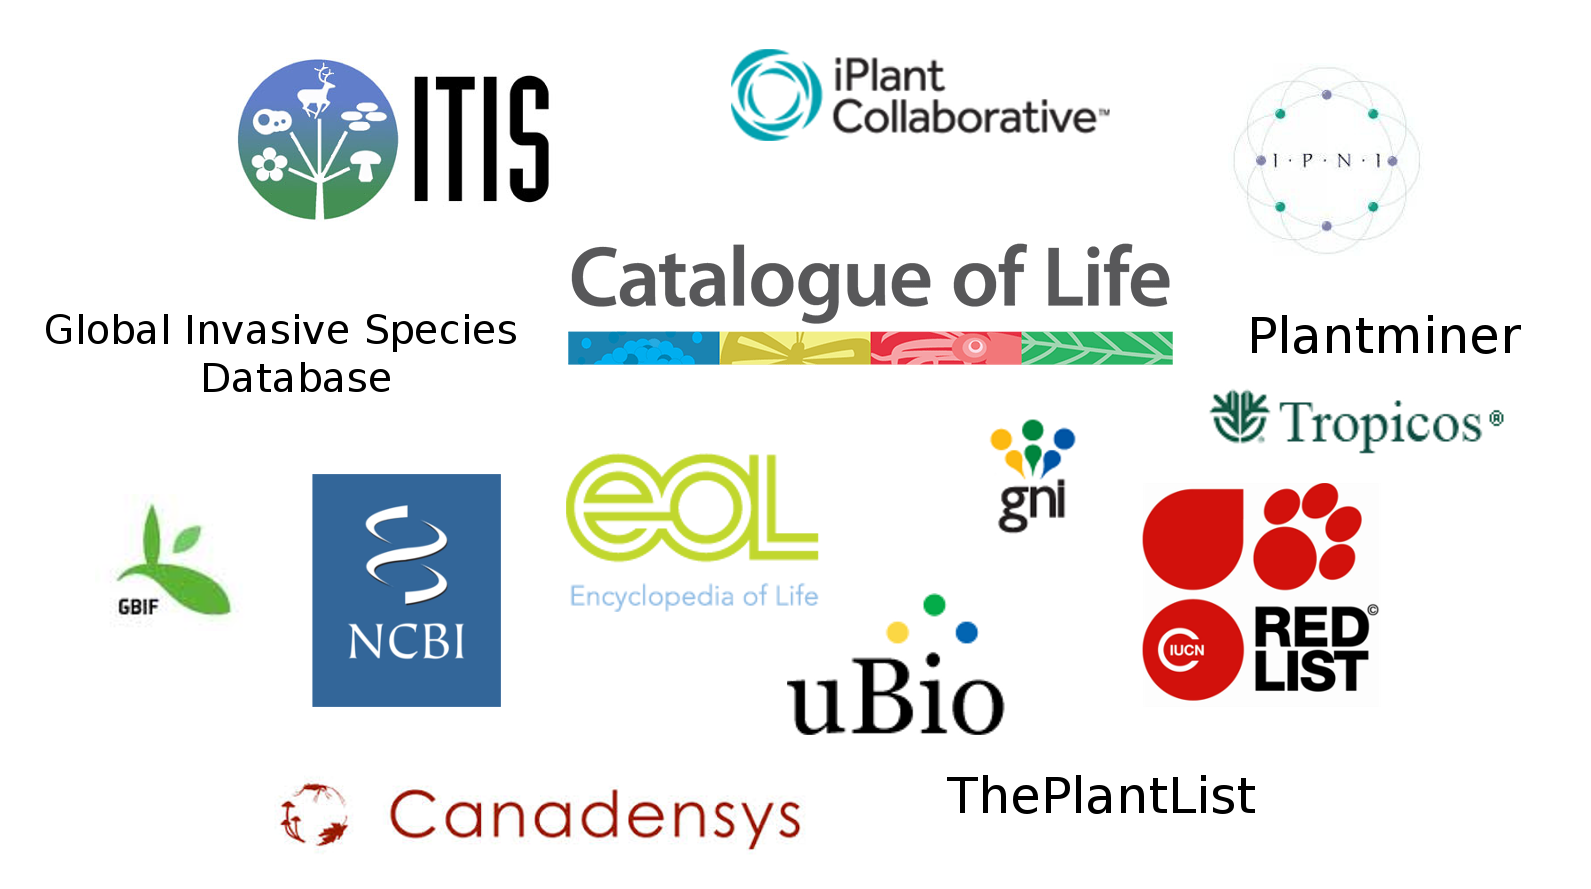
\includegraphics[width=0.8\linewidth]{fig/sources.png}
					\label{fig:sources}
				\end{figure}
			\end{block}

			\begin{block}{Features}
				\textcolor{i6bluedark}{\textbf{\large Resolve taxonomic names}}
        \vspace{0.5em}
        \par
        \begingroup
        \leftskip=2cm
        \noindent 
          We often have a list of species names and we want to know \\
          a) if we have the most up-to-date names, \\
          b) if our names are spelled correctly,  \\
          c) and the scientific name for a common name.\\
          Taxize provides an interface to the EOL Global Names Resolver and Taxonomic Name Resolution Service, e.g.
        \par
        \endgroup

\begin{knitrout}\footnotesize
\definecolor{shadecolor}{rgb}{0.933, 0.933, 0.933}\color{fgcolor}\begin{kframe}
\begin{alltt}
\hlkwd{gnr_resolve}\hlstd{(}\hlstr{'Baetis roodani'}\hlstd{)}
\end{alltt}
\end{kframe}
\end{knitrout}
\begin{knitrout}\footnotesize
\definecolor{shadecolor}{rgb}{0.933, 0.933, 0.933}\color{fgcolor}\begin{kframe}
\begin{verbatim}
##   submitted_name   matched_name
## 1 Baetis roodani Baetis rhodani
\end{verbatim}
\end{kframe}
\end{knitrout}
\vspace{2em}
					
\textcolor{i6bluedark}{\textbf{\large Retrieve higher taxonomic names}} 
        \vspace{0.5em}
        \par
        \begingroup
        \leftskip=2cm
        \noindent 
          One can also search in the opposite direction, i.e. search species within a genus:
        \par
        \endgroup

\begin{knitrout}\footnotesize
\definecolor{shadecolor}{rgb}{0.933, 0.933, 0.933}\color{fgcolor}\begin{kframe}
\begin{alltt}
\hlkwd{classification}\hlstd{(}\hlstr{'Baetis rhodani'}\hlstd{,} \hlkwc{db} \hlstd{=} \hlstr{'col'}\hlstd{)}
\end{alltt}
\end{kframe}
\end{knitrout}
\begin{knitrout}\footnotesize
\definecolor{shadecolor}{rgb}{0.933, 0.933, 0.933}\color{fgcolor}\begin{kframe}
\begin{verbatim}
##             name        rank
## 1       Animalia     Kingdom
## 2     Arthropoda      Phylum
## 3        Insecta       Class
## 4  Ephemeroptera       Order
## 5      Baetoidea Superfamily
## 6       Baetidae      Family
## 7         Baetis       Genus
## 8 Baetis rhodani     Species
\end{verbatim}
\end{kframe}
\end{knitrout}
\vspace{2em}


\textcolor{i6bluedark}{\textbf{\large Building taxonomic trees}} 
        \vspace{0.5em}
        \par
        \begingroup
        \leftskip=2cm
        \noindent 
          Using this taxonomic information we can build taxonomic trees. 
          The can be used a surrogates when phylogenetic data is scarce.
        \par
        \endgroup
\begin{knitrout}\footnotesize
\definecolor{shadecolor}{rgb}{0.933, 0.933, 0.933}\color{fgcolor}\begin{kframe}
\begin{alltt}
\hlstd{species} \hlkwb{<-} \hlkwd{c}\hlstd{(}\hlstr{"Juncus bufonius"}\hlstd{,} \hlstr{"Juncus articulatus"}\hlstd{,}
    \hlstr{"Aira praecox"}\hlstd{,} \hlstr{"Rumex acetosa"}\hlstd{,} \hlstr{"Baetis rhodani"}\hlstd{)}
\hlstd{hier} \hlkwb{<-} \hlkwd{classification}\hlstd{(species,} \hlkwc{db} \hlstd{=} \hlstr{'ncbi'}\hlstd{)}
\end{alltt}
\end{kframe}
\end{knitrout}

\begin{knitrout}\footnotesize
\definecolor{shadecolor}{rgb}{0.933, 0.933, 0.933}\color{fgcolor}\begin{kframe}
\begin{alltt}
\hlkwd{plot}\hlstd{(}\hlkwd{class2tree}\hlstd{(hier))}
\end{alltt}
\end{kframe}
\end{knitrout}
\vspace{2em}

\begin{knitrout}\footnotesize
\definecolor{shadecolor}{rgb}{0.933, 0.933, 0.933}\color{fgcolor}

{\centering 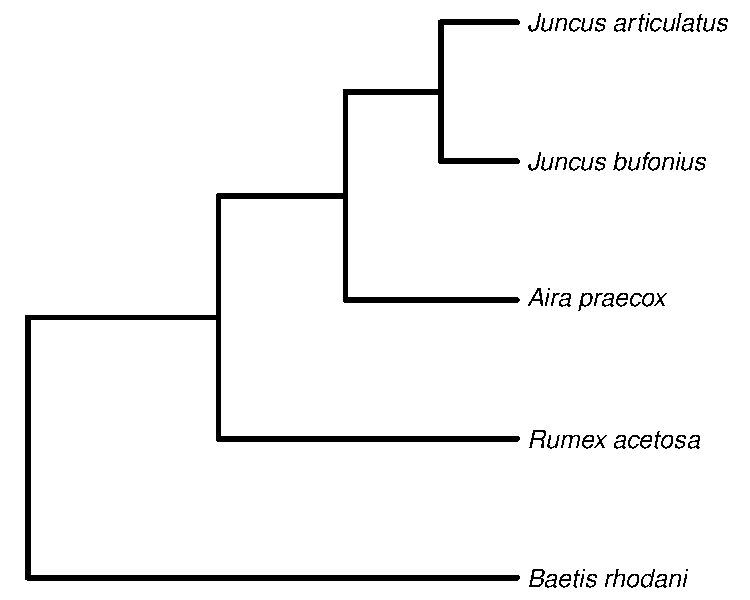
\includegraphics[width=0.4\linewidth]{figure/classtree} 

}



\end{knitrout}
\vspace{2em}

			\end{block}
		\end{column}
    
		\begin{column}{0.005\linewidth}
		\end{column}



		\begin{column}{.49\linewidth}
			\vspace{-\baselineskip}
      
      \begin{block}{Features (cont.)}
\textcolor{i6bluedark}{\textbf{\large Retrieve children taxa}}
        \vspace{0.5em}
        \par
        \begingroup
        \leftskip=2cm
        \noindent 
          Another common task is to retrieve the complete taxonomic hierarchy for a taxon:
        \par
        \endgroup
\begin{knitrout}\footnotesize
\definecolor{shadecolor}{rgb}{0.933, 0.933, 0.933}\color{fgcolor}\begin{kframe}
\begin{alltt}
\hlkwd{downstream}\hlstd{(}\hlstr{'Baetis'}\hlstd{,} \hlkwc{db} \hlstd{=} \hlstr{'col'}\hlstd{,} \hlkwc{downto} \hlstd{=} \hlstr{'Species'}\hlstd{)}
\end{alltt}
\end{kframe}
\end{knitrout}
\begin{knitrout}\footnotesize
\definecolor{shadecolor}{rgb}{0.933, 0.933, 0.933}\color{fgcolor}\begin{kframe}
\begin{verbatim}
##      childtaxa_name childtaxa_rank
## 1   Baetis acceptus        Species
## 2  Baetis aculeatus        Species
## 3 Baetis acuminatus        Species
## 4     Baetis adonis        Species
## 5     Baetis aeneus        Species
\end{verbatim}
\end{kframe}
\end{knitrout}
\vspace{2em}

\textcolor{i6bluedark}{\textbf{\large Aggregate data to a specific taxonomic rank}}
        \vspace{0.5em}
        \par
        \begingroup
        \leftskip=2cm
        \noindent 
          Using the taxonomic information taxa can be easily aggregated to different levels, e.g. to study effects on different taxonomic levels.
          This is provided via the \texttt{tax\_agg()} function:
        \par
        \endgroup

\begin{knitrout}\footnotesize
\definecolor{shadecolor}{rgb}{0.933, 0.933, 0.933}\color{fgcolor}\begin{kframe}
\begin{alltt}
\hlkwd{tax_agg}\hlstd{(dune,} \hlkwc{rank} \hlstd{=} \hlstr{'family'}\hlstd{,} \hlkwc{db} \hlstd{=} \hlstr{'ncbi'}\hlstd{)}
\end{alltt}
\end{kframe}
\end{knitrout}
\vspace{2em}

\textcolor{i6bluedark}{\textbf{\large Match tables with different taxonomic resolution}}
        \vspace{0.5em}
        \par
        \begingroup
        \leftskip=2cm
        \noindent 
          Using the taxonomic information taxa can be easily aggregated to different levels, e.g. to study effects on different taxonomic levels.
          This is provided via the \texttt{tax\_agg()} function:
        \par
        \endgroup

\begin{knitrout}\footnotesize
\definecolor{shadecolor}{rgb}{0.933, 0.933, 0.933}\color{fgcolor}\begin{kframe}
\begin{alltt}
\hlkwd{tax_agg}\hlstd{(dune,} \hlkwc{rank} \hlstd{=} \hlstr{'family'}\hlstd{,} \hlkwc{db} \hlstd{=} \hlstr{'ncbi'}\hlstd{)}
\end{alltt}
\end{kframe}
\end{knitrout}
\vspace{2em}
      \end{block}
      
      \begin{block}{Under the hood}
      
      \end{block}
      
			\begin{block}{Get involved!}
				\begin{columns}[T]
					\begin{column}{.78\linewidth}
						taxize is currently developed collaboratively in github. Feature requests, bug reports and contributions are strongly encouraged! \\[0.5em]
						\huge \Mundus \normalsize \hspace{0.5cm} https://github.com/ropensci/taxize
					\end{column}
					\begin{column}{.2\linewidth}
						
\includegraphics[width=0.85\linewidth]{fig/github.png}
					\end{column}
				\end{columns}
			\end{block}
		\end{column}
	\end{columns}
\end{frame}
\end{document}
